\chapter*{Introduction}

\addcontentsline{toc}{chapter}{Introduction}

This work focuses on the mathematical modeling of fluid flow, with an emphasis on optimizing the shape of walls of the idealized total cavopulmonary connection (TCPC). In many engineering fields such as the automotive or aerospace industries, incorporating optimization processes to find the optimal shape of the studied object is a standard practice. In clinical medicine, however, the use of optimization techniques  is less common due to various challenges. Accurate modeling of blood flow, often through complex geometries, requires careful validation against experimental data, which can be difficult to obtain -- \textit{in vivo} (in a living organism) experiments are naturally often infeasible or ethically constrained, complicating the process of validation.

Nevertheless, the process of shape optimization can find great potential especially in cardiac and vascular surgery \cite{Abraham2005, Weddell2015, Marsden2008, Sharma1996, Ensley1999}. Developing a systematic optimization framework for medical applications would provide clinicians with an \textit{in vitro} (outside a living organism) tool to assess surgical procedures within patient-specific geometries. Designing and implanting objects such as stents or artificial valves could then be directly tailored to the patient's anatomy. This approach could lead to improved clinical outcomes, reduced risk of postoperative complications, and a general improvement in the patient's quality of life \cite{Marsden2008, Rijnberg2018}.

An example of a specific surgical procedure where the process of wall shape optimization can find its application is the total cavopulmonary connection. TCPC is performed on children diagnosed with a congenital heart defect reffered to as functionally single ventricle, where  the heart can effectively utilize only one functional ventricle for the blood circulation \cite{Chaloup}. In this procedure, the superior vena cava (\textit{vena cava superior}, labeled \textit{d} in Figure~\ref{fig:tcpc}) is surgically connected to the pulmonary artery. The inferior vena cava (\textit{vena cava inferior}, labeled \textit{b} in Figure~\ref{fig:tcpc}) is also connected directly to the pulmonary artery (\textit{arteria pulmonalis}, labeled \textit{a} in Figure~\ref{fig:tcpc}), typically using an extracardiac conduit (labeled \textit{c} in Figure~\ref{fig:tcpc}), which is a vascular prosthesis \cite{Rubtsova, Delorme}.

\begin{figure}[h]
	\centering
	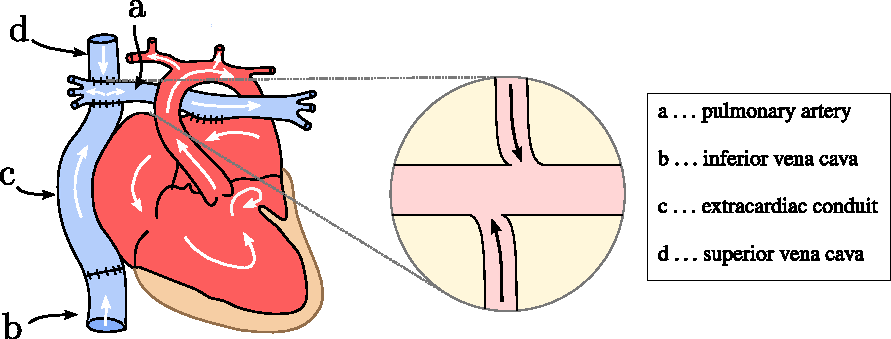
\includegraphics[width=0.97\textwidth]{figures/heart.pdf}
	\vspace{5mm}
	\caption{Diagram of the total cavopulmonary connection. The enlarged region shows the extracardiac conduit connection.}
	\label{fig:tcpc}

\end{figure}

While TCPC enables functional blood circulation, the resulting circulatory system is highly sensitive to energy losses caused by factors such as turbulent flow and flow collisions. These inefficiencies can gradually lead to system failure. The shape of the extracardiac conduit connection, aiming to minimize energy losses or tissue stress, is therefore well-suited to be a subject of optimization \cite{Chaloup, vanBake, Wang}. Numerous studies address the issue of optimal conduit connection, however, many explore and examine only a small number of geometry variations using a "trial-and-error” approach rather than a rigorous optimization process \cite{Ensley1999, Rijnberg2018, Porfiryev2020, Tang2014}.

To create an optimization framework usable in the context of blood flow simulations, it is necessary to use an efficient and reliable numerical method to compute the values of the objective function, which is subject to minimization.  In this work, the lattice Boltzmann method (LBM) is used for numerical computations. Note that an in-house implementation of LBM developed at the Department of Mathematics of FNSPE CTU in Prague was used and modified according to the needs of this work. The main advantage of LBM is the possibility of massive parallelization on GPUs (graphics processing units), which can potentially significantly reduce the computational time compared to standard numerical methods for fluid flow modeling \cite{PE, Kruger}.

However, LBM also has a notable limitation in the context of geometry representation. The method relies on a regular grid for spatial discretization, which results in a stair-step approximation of boundaries, which can pose challenges when modeling complex geometries such as blood vessels. To address this challenge, previous work \cite{buresBP, buresVU} studied the implementation of interpolated boundary conditions, enabling more accurate representation of boundary shapes within LBM. Furthermore, \cite{buresVU} explored the coupling of both gradient-based and gradient-free optimization methods with LBM. The results from \cite{buresVU} indicate that gradient-free optimization methods are more suitable in the context of this work, making the implementation of interpolated boundary conditions unnecessary for the optimization process to proceed effectively.

The structure of this work is organized as follows. The first chapter introduces the mathematical model of fluid flow, with a focus on modeling of blood flow in vessels. The second chapter provides discusses the numerical method employed, the lattice Boltzmann method. The third chapter details the custom tool developed for efficient parameterization and automatic generation of 3D geometries, tailored to the requirements of the optimization process. The fourth chapter introduces the theory of mathematical optimization and details the optimization methods utilized in this work. Additionally, this chapter introduces the proposed optimization framework. The final chapter presents the results of the numerical experiments. First, the optimization framework is validated on a simplified test problem involving a cylinder junction with a single optimization parameter, inspired by an idealized 3D model of TCPC. Then, optimization is applied to more complex problems based on an extended 3D idealized model of TCPC, incorporating multiple optimization parameters. Among other things, the influence of different optimization methods and objective functions on the performance and outcomes of the optimization framework is examined.


